\documentclass[a4paper, 12pt, twoside]{report}

\usepackage{physics, amsmath, amsfonts, siunitx}
\usepackage{tcolorbox}
\usepackage{todonotes}
\usepackage{enumitem}
\usepackage{hyperref}
\usepackage{graphicx}
\graphicspath{ {./ch1} }
\hypersetup{
    colorlinks=true,
    linkcolor=blue,
    urlcolor=blue,
}

\usepackage{geometry}
\geometry{
    top=2cm,
    bottom=2cm,
    left=2cm,
    right=3cm,
    headheight=17pt,
    includeheadfoot,
}

\usepackage{fancyhdr, lastpage}
\pagestyle{fancy}
\cfoot{Page \thepage\ of \pageref{LastPage}}
\usepackage{graphicx} % Required for inserting images

\usepackage{etoolbox}
\patchcmd{\chapter}{\thispagestyle{plain}}{\thispagestyle{fancy}}{}{}

\title{Quantum Computing}
\author{Pietro Garofalo \\ Jasmine Amani Murphy}
\date{\today}


\begin{document}

\maketitle
\newpage
\listoftodos
\newpage
\tableofcontents
\newpage

\chapter*{Introduction}
Hi everyone, this work is a simple collection of notes taken during the Womanium Global Quantum program, our goal is to try to share as much as possible what we learned during the course and not only : the document is open-source so anyone can participate in the writing or just correct any mistakes, the repository can be found \href{https://github.com/Jazy1618/Quantum-Notebook}{here}.

\newpage

\chapter{Single Qbit and superposition principle}
When we are talking about a qbit we are referring to a quantum state and in order to describe it mathematically we need a vector space called Hilbert space.\\
In the simplest case of a single qbit we define our " computational basis " as follows using the Dirac notation: 
\begin{align*}
    \ket{0} = \begin{pmatrix}1\\0\end{pmatrix} && \ket{1} = \begin{pmatrix}0 \\ 1\end{pmatrix} 
\end{align*}  
As the classical case our qbit can  be in either the state $\ket{0}$ or the $\ket{1}$, the difference is a fundamental principle of quantum mechanics called \textit{Quantum superposition}: in classical mechanics things are well defined however in quantum mechanics the state of a particle ( our qbit ) can be write as the linear combination of other states, in other words a sum of two or more states gives as result another valid state

\begin{equation*}
    \ket{\psi} = \alpha \ket{0} + \beta \ket{1} = \begin{pmatrix} \alpha \\ \beta \end{pmatrix}
\end{equation*}

\section{Quantum logic gates}
In quantum circuits we can perform operations to the qbits through what are called \textit{Quantum logical gates} represented as unitary matrices. \\
In order to understand their effects to a qbit is easier to give some examples of the most important ones.
\subsection{The NOT gate X}

\chapter{Multistate qbit}

\newpage

\chapter{Quantum Algorithms}
For many students, practice is the best way to learn so in this chapter we study  some quantum algorithms.  
\section{Deutsch-Jozsa Algorithm}
The problem is : given a function $\textit{f} : \{0,1\}^n \rightarrow \{0,1\}$ whose definition in unknown, determine whether that function is constant or balanced, knowing for certain that $\textit{f}$ will be either constant or balanced. \\
What does it mean? Well $\textit{f}$ is just a machine that "eats" a string of length $n$ composed by 0 and 1, and spits out either a 0 or a 1, lets do and example with just 2 bits : 

\begin{center}
\begin{tabular}{|c|c|}
\hline
$\{0,1\}^2$ & \textit{f} \\
\hline
  00   & 1 \\
\hline
   01  &  1 \\
   \hline
   10 & 0 \\
   \hline
   11 & 0 \\
   \hline
\end{tabular}
\quad
\begin{tabular}{|c|c|}
\hline
$\{0,1\}^2$ & \textit{f} \\
\hline
  00   & 1 \\
\hline
   01  &  1 \\
   \hline
   10 & 1 \\
   \hline
   11 & 1 \\
   \hline
\end{tabular}   
\end{center}
In the example above each row of the tables represent a " question " asked to the oracle, we have 2 bits so $\{0,1\}^2$ is a string of length 2, the whole set is in general of dimension $2^n$ so in our case we can create four different combinations. \\
We can notice that the table on the left represents a balanced function in fact as output it gives the exact same number of 0 and 1, the table on the right represents a constant function. \\
It is easy to see that in order to be sure about the nature of our function, if we have $n$ bits,we have to ask a number of questions equal to half plus one of the size of our set : $2^{n-1} + 1$, in contrast in the quantum case we will see how we need only ask one question. \\ 
We start by implementing the algorithm for 2 qbits and then we can generalize for $n$ qbit.
\newpage
\subsection{Implementation for two qbits}
\textit{By making mistakes we learn}, we will implement the Deutsch algorithm by trial and error.
As we can see in figure \ref{Deutsh2Bits} we start with two bits both at state $\ket{0}$, since the oracle calculates \textit{f} on the first qbit, in order to maximize the potential of qbits we apply the Hadamard gate to the first qbit so that we have a state in superposition. \\
\begin{figure}[h]
    \centering
    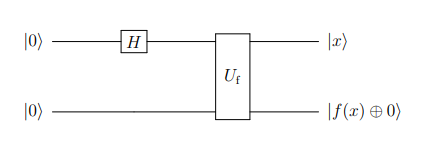
\includegraphics{QuantumAlgorithms/images/Deutsch2Bits.png}
    \caption{\todo{caption}}
    \label{Deutsh2Bits}
\end{figure}
\\
We denote the state after the i-th operation $\ket{\psi_i}$. \\
So we have the initial state : 
\begin{align*}
    \ket{\psi_1} = \ket{00} = \begin{pmatrix}1 \\ 0 \\ 0 \\ 0\end{pmatrix}
\end{align*}
After applying the hadamard gate to the first qbit we have :
\begin{align*}
    \ket{\psi_2} &= H\ket{0} \otimes \mathbb{I}\ket{0} \\[10pt]
    &= \qty(\frac{\ket{0} + \ket{1}}{\sqrt{2}})\ket{0} \\[10pt]
    &= \frac{\ket{00} + \ket{10}}{\sqrt{2}}
\end{align*}
At the end of our circuit we have : 
\begin{align*}
    \ket{\psi_3} &= \frac{\ket{0,f(0)\oplus 0} + \ket{1, f(1) \oplus 0}}{\sqrt{2}} \\[10pt]
    &= \frac{\ket{0,f(0)} + \ket{1,f(1)}}{\sqrt{2}}
\end{align*}
\newpage
Effectively our circuit calculates what we need, the problem is that the final state is kept in superposition so measuring it we would have a 50\% chance of having \textit{f(0)} and 50\% chance of having \textit{f(1)}. \\
Let's try another approach, we set the second qbit to 1 and apply hadamard gate to it, to be as general as possible the first is set to any state

\begin{figure}[h]
    \centering
    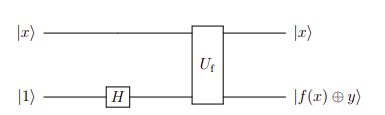
\includegraphics{QuantumAlgorithms/images/Deutsch2Bit2.png}
    \label{Deutsh2Bits2}
\end{figure}

\begin{align*}
    \ket{\psi_2} &= \ket{x} \otimes H\ket{1} \\[10pt]
                 &= \frac{\ket{x,0} - \ket{x,1}}{\sqrt{2}}
\end{align*}

\newpage



\chapter{Qbit Hardware}
In the previous chapter we saw several examples of the kinds of algorithms that can become possible by leveraging quantum technologies with information processing. To take these algorithms from theory to actualization will require a physical quantum computer capable of performing various calculations on a system of stable qbits. An active area of research in quantum computing is deciding what physical system is best able to model the quantum nature of a qbit, particularly based on the Di Vincenzo’s criteria.

In this chapter we'll go over several of the leading hardware solutions to building a universal gate quantum computer, and at the end compare their pros and cons as it relates to the Di Vincenzo criteria.

\section{Quantum Annealers}
Before we get into creating quantum computers, Let's discuss anther device that has come a long way in recent decades - the quantum annealer. A quantum annealer is a device designed for optimizing solutions to a single type of problem by quickly searching over a space and finding a solution. 

\section{Neutral-Atom Quantum Computers}

\section{Superconducting Quantum Computers}

\section{Photonic Quantum Computers}

\section{Silicon-based Quantum Computers}

\section{Trapped-Ion Quantum Computers}

\section{Summary}


\chapter{Quantum Key Distribution}
When Peter Shor introduced his now famous Shor's algorithm in the 1990s, it spelled the end of RSA and other factorization-based encryption methods. It was an unofficial call to kick the quantum computing race into high gear - although not all for the same reasons. Suddenly there was an awareness that this technology could devastate the security of various important sectors by rendering their encryption methods useless. With this issue becoming very apparent over time, 
In light of the capabilities of a fully realized quantum computer, there are certain security concerns that become realized



\end{document}
